\section{}
\[
H(s)=\frac{s+1}{(s+10)^2}\,.
\]
\subsection{Bode-Diagramm}
\begin{center}
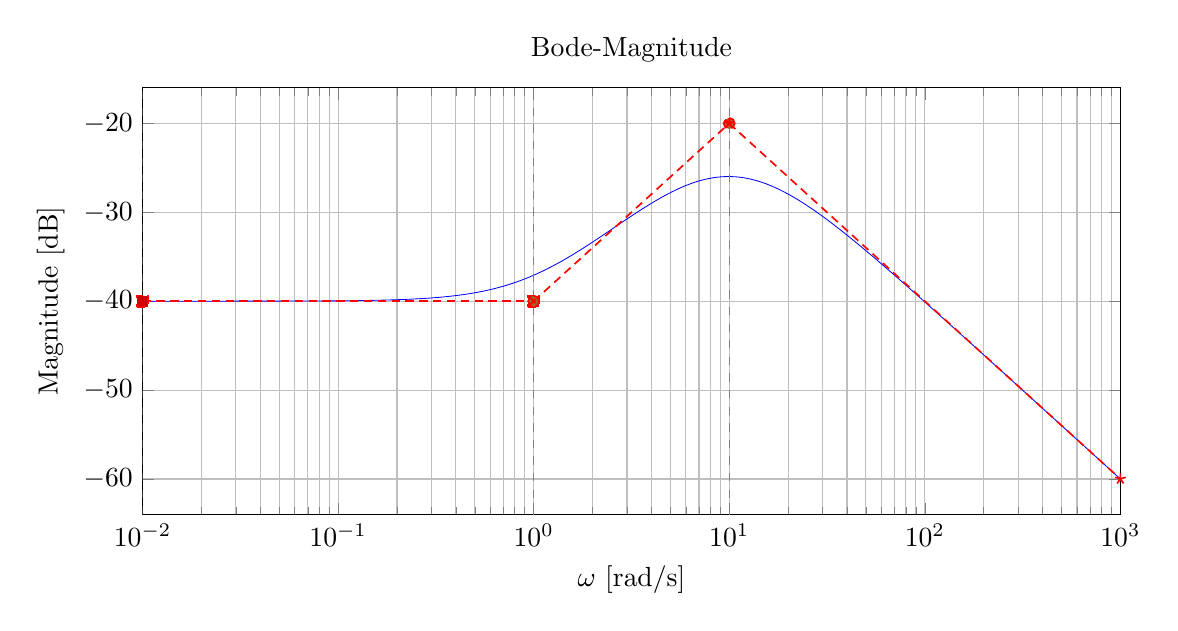
\begin{tikzpicture}
\begin{semilogxaxis}[
  width=14cm,height=7cm,
  xmin=1e-2,xmax=1e3,
  xlabel={$\omega$ [rad/s]},
  ylabel={Magnitude [dB]},
  grid=both,
  title={Bode-Magnitude}
]
\addplot[
  domain=1e-2:1e3,
  samples=600,
  mark=none,
  line width=0.3pt,
  blue
] {20*ln(sqrt(1 + x^2))/ln(10) - 40*ln(sqrt(100 + x^2))/ln(10)};
\addplot+[domain=1e-2:1,samples=2,dashed,dash pattern=on 3pt off 2pt,line width=0.6pt,red] {-40};
\addplot+[domain=1:1e1,samples=2,dashed,dash pattern=on 3pt off 2pt,line width=0.6pt,red] {-40 + 20*ln(x)/ln(10)};
\addplot+[domain=1e1:1e3,samples=2,dashed,dash pattern=on 3pt off 2pt,line width=0.6pt,red] {-20 - 20*ln(x/10)/ln(10)};
\draw[gray,dashed] (rel axis cs:0,0) -- (rel axis cs:0,1);
\draw[gray,dashed] (axis cs:1,\pgfkeysvalueof{/pgfplots/ymin}) -- (axis cs:1,\pgfkeysvalueof{/pgfplots/ymax});
\draw[gray,dashed] (axis cs:10,\pgfkeysvalueof{/pgfplots/ymin}) -- (axis cs:10,\pgfkeysvalueof{/pgfplots/ymax});
\node[gray,anchor=south east] at (axis cs:1,\pgfkeysvalueof{/pgfplots/ymax}) {\scriptsize Nullstelle $\omega_z=1$};
\node[gray,anchor=south east] at (axis cs:10,\pgfkeysvalueof{/pgfplots/ymax}) {\scriptsize Pol $\omega_p=10$ (doppelt)};
\end{semilogxaxis}
\end{tikzpicture}
\vspace{6mm}
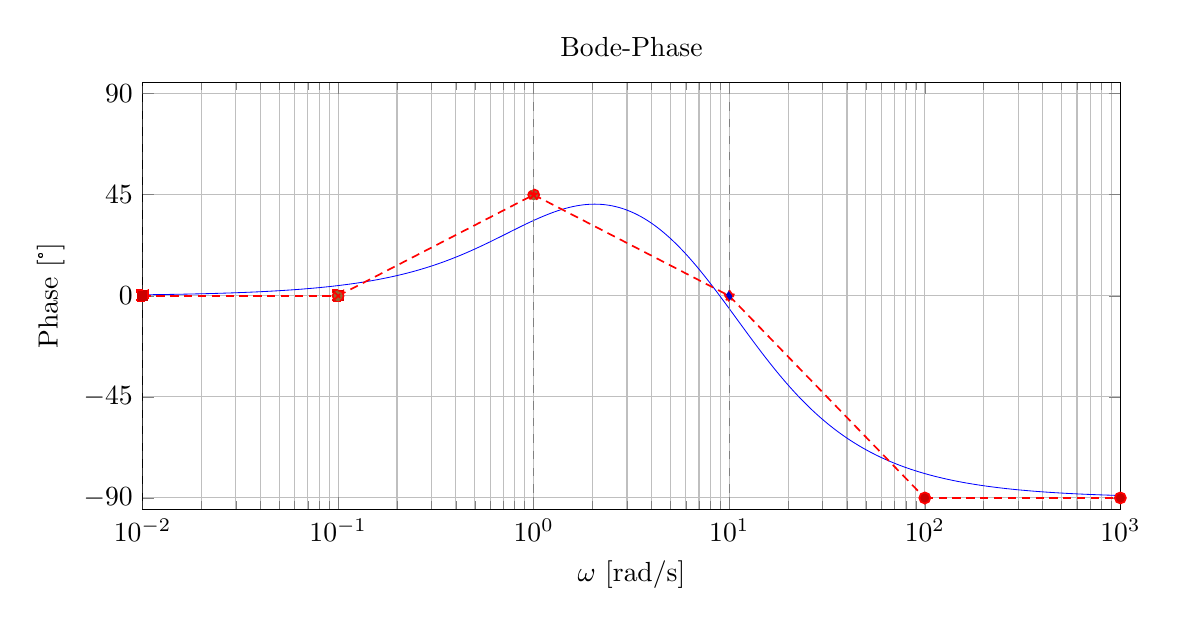
\begin{tikzpicture}
\begin{semilogxaxis}[
  width=14cm,height=7cm,
  xmin=1e-2,xmax=1e3,
  ytick distance=45,
  ymin=-95,ymax=95,
  xlabel={$\omega$ [rad/s]},
  ylabel={Phase [°]},
  grid=both,
  title={Bode-Phase}
]
\addplot[
  domain=1e-2:1e3,
  samples=600,
  mark=none,
  line width=0.3pt,
  blue
] {atan(x) - 2*atan(x/10)};
\addplot+[domain=1e-2:1e-1,samples=2,dashed,dash pattern=on 3pt off 2pt,line width=0.6pt,red] {0};
\addplot+[domain=1e-1:1e0,samples=2,dashed,dash pattern=on 3pt off 2pt,line width=0.6pt,red] {45 + 45*ln(x)/ln(10)};
\addplot+[domain=1e0:1e1,samples=2,dashed,dash pattern=on 3pt off 2pt,line width=0.6pt,red] {45 - 45*ln(x)/ln(10)};
\addplot+[domain=1e1:1e2,samples=2,dashed,dash pattern=on 3pt off 2pt,line width=0.6pt,red] {-90*ln(x/10)/ln(10)};
\addplot+[domain=1e2:1e3,samples=2,dashed,dash pattern=on 3pt off 2pt,line width=0.6pt,red] {-90};
\draw[gray,dashed] (rel axis cs:0,0) -- (rel axis cs:0,1);
\draw[gray,dashed] (axis cs:1,\pgfkeysvalueof{/pgfplots/ymin}) -- (axis cs:1,\pgfkeysvalueof{/pgfplots/ymax});
\draw[gray,dashed] (axis cs:10,\pgfkeysvalueof{/pgfplots/ymin}) -- (axis cs:10,\pgfkeysvalueof{/pgfplots/ymax});
\node[gray,anchor=south east] at (axis cs:1,\pgfkeysvalueof{/pgfplots/ymax}) {\scriptsize Nullstelle $\omega_z=1$};
\node[gray,anchor=south east] at (axis cs:10,\pgfkeysvalueof{/pgfplots/ymax}) {\scriptsize Pol $\omega_p=10$ (doppelt)};
\end{semilogxaxis}
\end{tikzpicture}
\end{center}
\newpage
\subsection{Erklärung}
\begin{description}[leftmargin=1.2em,labelsep=.6em,font=\bfseries]

\item[1. Normalform herstellen.]
Bringe die Übertragungsfunktion exakt in die im Skript definierte Standardform.
\[
H(s)=\frac{s+1}{(s+10)^2}
= K_0\cdot(1+sT_z)\cdot\frac{1}{(1+sT_p)^2}
\]
mit
\[
K_0=\frac{1}{100},\quad r=0,\quad T_z=1,\quad T_p=\tfrac{1}{10}.
\]
\[
\underline{F}_1(s)=1+sT_z\quad\text{(LHP-Nullstelle)},\qquad
\underline{F}_2(s)=\frac{1}{(1+sT_p)^2}\quad\text{(Doppelpol)}.
\]

\item[2. Eckfrequenzen bestimmen und sortieren.] Die $\omega$-Eckfrequenzen lassen sich aus den $T_n$'s bestimmen und müssen anschließend sortiert werden:
\[
\omega_z=\frac{1}{T_z}=1\,\mathrm{rad/s},\qquad \omega_p=\frac{1}{T_p}=10\,\mathrm{rad/s},\qquad \omega_z<\omega_p.
\]

\item[3. Startpunkt des Amplitudengangs festlegen (Geradennäherung).]
Setze \(\omega_{\min}=\omega_z=1\).
\[
F_{\mathrm{dB}}(\omega_{\min})=20\log_{10}\!\Big(|K_0F^*_{ges}(0)|\,\omega_{\min}^{\,r}\Big)
=20\log_{10}\!\Big(\frac{1}{100}\cdot 1\cdot 1^{0}\Big)=-40\,\mathrm{dB}.
\]
Ankerpunkt: \(-40\,\mathrm{dB}\) bei \(\omega=1\).

\item[4. Verlauf links vom Startpunkt zeichnen.]
Für \(\omega<1\): Anfangssteigung \(r\cdot 20=0\,\mathrm{dB/dec}\) \(\Rightarrow\) horizontale Asymptote bei \(-40\,\mathrm{dB}\).

\item[5. Steigungswechsel an den Eckfrequenzen eintragen.]
Nullstelle bei \(\omega_z=1\): \(+20\,\mathrm{dB/dec}\) ab \(\omega=1\).
Doppelpol bei \(\omega_p=10\): zusätzlich \(-40\,\mathrm{dB/dec}\) ab \(\omega=10\), also insgesamt \(-20\,\mathrm{dB/dec}\).
Netto:
\[
\begin{cases}
-40\,\mathrm{dB}\ \text{(flach)},& \omega<1,\\
-40+20\log_{10}\omega,& 1\le \omega<10\ \text{(Steigung }+20\,\mathrm{dB/dec}),\\
-20-20\log_{10}(\omega/10),& \omega\ge 10\ \text{(Steigung }-20\,\mathrm{dB/dec}).
\end{cases}
\]

\item[6. Eckabrundung korrekt berücksichtigen.]
LHP-Nullstelle: bei \(\omega=1\) liegt der exakte Betrag um \(+3\,\mathrm{dB}\) über der Gerade:
\[
|H(j1)|_{\mathrm{dB}}=10\log_{10}2-20\log_{10}101\approx -37\,\mathrm{dB}.
\]
Doppelpol: bei \(\omega=10\) insgesamt \(-6\,\mathrm{dB}\) unter der Asymptote:
\[
|H(j10)|_{\mathrm{dB}}=10\log_{10}101-20\log_{10}200\approx -26\,\mathrm{dB}.
\]

\item[7. Phasenstartwert festlegen.]
Da \(K_0\underline{F}_{ges}^*(0)>0\), \(r=0\) \(\Rightarrow\) \(\varphi(0)=r\cdot90^\circ=0^\circ\).

\item[8. Phasenänderung durch Nullstelle und Doppelpol eintragen.]
Nullstelle bewirkt eine Phasenänderung um \(+90^\circ\) über \([0.1,10]\). Jeder Pol \(-90^\circ\) über \([1,100]\) (zwei Pole \(\Rightarrow -180^\circ\) total). Die Effekte überlappen sich in $[1,10]$; dort addieren sich die Steigungen.
Näherung:
\[
\varphi(\omega)\approx
\begin{cases}
0^\circ,& \omega\le 0.1,\\
45^\circ+45^\circ\log_{10}\omega,& 0.1<\omega<1,\\
45^\circ-45^\circ\log_{10}\omega,& 1<\omega<10,\\
-90^\circ\log_{10}(\omega/10),& 10<\omega<100,\\
-90^\circ,& \omega\ge 100.
\end{cases}
\]

\item[9. Grenzwerte und Konsistenz prüfen.]
DC: \(|H(0)|=\tfrac{1}{100}\Rightarrow -40\,\mathrm{dB}\), \(\varphi(0)=0^\circ\).
HF: \(|H(j\omega)|\sim \omega/\omega^2=1/\omega\Rightarrow -20\log_{10}(\omega/10)-20\,\mathrm{dB}\).
Pol-/Nullzählung: \(m=1\), \(n=2\Rightarrow (m-n)\cdot 90^\circ=-90^\circ\) \(\Rightarrow \varphi(\infty)=-90^\circ\).

\end{description}

\subsubsection*{Stückweise Näherungen (für die Skizze)}
\[
|H(j\omega)|_{\mathrm{dB}}\approx
\begin{cases}
-40,& \omega\ll 1,\\[2pt]
-40+20\log_{10}\omega,& 1\ll\omega\ll 10,\\[2pt]
-20-20\log_{10}(\omega/10),& \omega\gg 10,
\end{cases}
\]\[
\varphi(\omega)\approx
\begin{cases}
0^\circ,& \omega\le 0.1,\\[2pt]
45^\circ+45^\circ\log_{10}\omega,& 0.1<\omega<1,\\[2pt]
45^\circ-45^\circ\log_{10}\omega,& 1<\omega<10,\\[2pt]
-90^\circ\log_{10}(\omega/10),& 10<\omega<100,\\[2pt]
-90^\circ,& \omega\ge 100.
\end{cases}
\]

\newpage